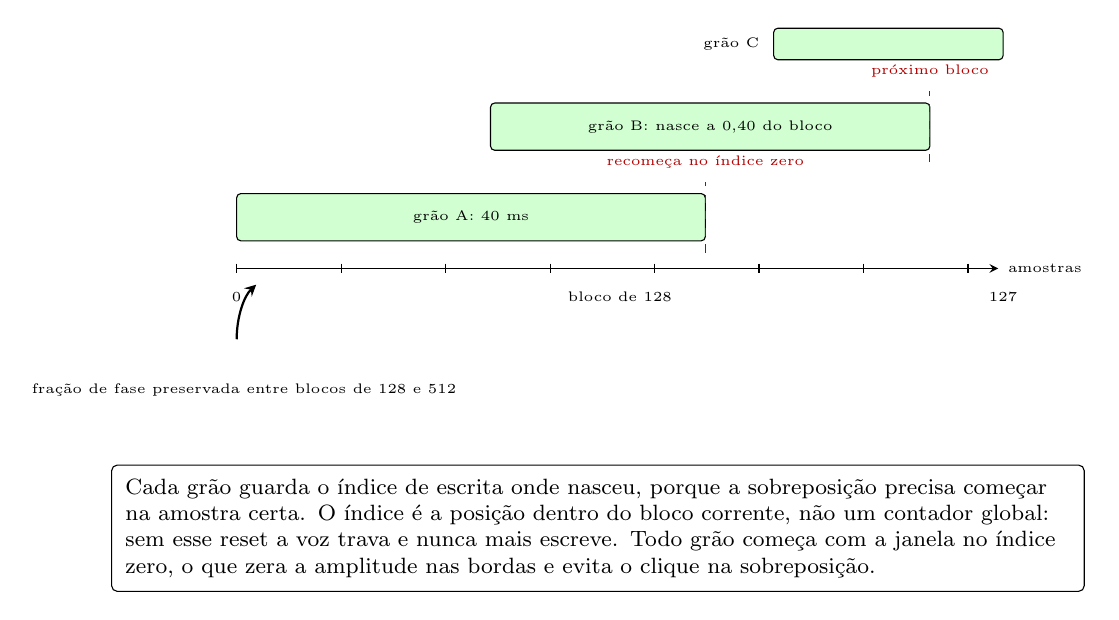
\begin{tikzpicture}[x=0.62cm]
  \tikzstyle{g}=[fill=green!18, draw, rounded corners=1.5pt]
  \tikzstyle{cut}=[draw, red!70!black, dashed]
  \tikzstyle{lab}=[font=\tiny, fill=white, inner sep=1.5pt]

  % linha do tempo de amostras de um bloco
  \draw[->, >=stealth] (0,0) -- (15.6,0) node[right, font=\tiny] {amostras};
  \foreach \x in {0,2.14,...,15.7} {
    \draw (\x,0.06) -- (\x,-0.06);
  }
  \node[font=\tiny, anchor=north] at (0,-0.18) {0};
  \node[font=\tiny, anchor=north] at (7.85,-0.18) {bloco de 128};
  \node[font=\tiny, anchor=north] at (15.7,-0.18) {127};

  % grao A: nasce no inicio e sobrevive ao bloco
  \fill[g] (0,0.35) rectangle (9.6,0.95);
  \node[font=\tiny] at (4.8,0.65) {grão A: 40 ms};
  \draw[cut] (9.6,0.2) -- (9.6,1.1);
  \node[font=\tiny, text=red!70!black, anchor=south] at (9.6,1.15) {recomeça no índice zero};

  % grao B: nasce no meio do bloco
  \fill[g] (5.2,1.5) rectangle (14.2,2.1);
  \node[font=\tiny] at (9.7,1.8) {grão B: nasce a 0,40 do bloco};
  \draw[cut] (14.2,1.35) -- (14.2,2.25);
  \node[font=\tiny, text=red!70!black, anchor=south] at (14.2,2.3) {próximo bloco};

  % grao C: esparso, com densidade baixa
  \fill[g] (11.0,2.65) rectangle (15.7,3.05);
  \node[font=\tiny, anchor=east] at (10.9,2.85) {grão C};

  % anotacao da fracao de fase
  \draw[->, >=stealth, thick] (0,-0.9) arc[start angle=180, end angle=120, radius=0.8];
  \node[lab] at (0.15,-1.55) {fração de fase preservada entre blocos de 128 e 512};

  % nota de amplitude
  \node[draw, fill=white, rounded corners=2pt, align=left, font=\footnotesize, inner sep=5pt, text width=12.0cm] at (7.4,-3.3)
    {Cada grão guarda o índice de escrita onde nasceu, porque a sobreposição precisa começar na amostra certa. O índice é a posição dentro do bloco corrente, não um contador global: sem esse reset a voz trava e nunca mais escreve. Todo grão começa com a janela no índice zero, o que zera a amplitude nas bordas e evita o clique na sobreposição.};
\end{tikzpicture}
